\documentclass[letterpaper,12pt]{article}
\usepackage{tabularx} % extra features for tabular environment
\usepackage{amsmath}  % improve math presentation
\usepackage{graphicx} % takes care of graphic including machinery
\usepackage[margin=0.95in,letterpaper]{geometry} % decreases margins
\usepackage{cite} % takes care of citations
\usepackage[titletoc,title]{appendix} % takes care of appendices
\usepackage{listings} % code representation
\usepackage{pdflscape}
\usepackage{csquotes} % for quoting existing work
\usepackage{color} % defines colors for code listings
\usepackage{comment} % allows for block of comments
\usepackage{gensymb} % degree symbol
\usepackage{rotating} % horizontal figure
\usepackage[final]{hyperref} % adds hyper links inside the generated pdf file

% style code listings
\definecolor{codegreen}{rgb}{0,0.6,0}
\definecolor{codegray}{rgb}{0.5,0.5,0.5}
\definecolor{backcolour}{rgb}{0.95,0.95,0.92}
\lstdefinestyle{mystyle}{
    backgroundcolor=\color{backcolour},   
    commentstyle=\color{codegreen},
    keywordstyle=\color{blue},
    numberstyle=\tiny\color{codegray},
    basicstyle=\footnotesize,
    breakatwhitespace=false,         
    breaklines=true,                 
    captionpos=b,                    
    keepspaces=true,                 
    numbers=left,                    
    numbersep=5pt,                  
    showspaces=false,                
    showstringspaces=false,
    showtabs=false,                  
    tabsize=4
}
\lstset{style=mystyle}

\begin{document}

\title{CS5011 Artificial Intelligence Practice\\Practical 1 Report}
\author{Student ID: 150014151}
\date{11 October, 2019}
\maketitle
\newpage


% --------------------------------------- 1 - INTRODUCTION ------------------------------------------ 

\section{Introduction}
\label{sec:introduction}

The Advanced Agent was attempted for this Practical. The following features were implemented:
\begin{itemize}
    \item Basic Agent:
    \begin{itemize}
       \item Breadth-First Search
        \item Depth-First Search
    \end{itemize}
    \item Intermediate Agent:
    \begin{itemize}
        \item Best-First Search
        \item A* Search
    \end{itemize}
    \item Advanced Agent (1 extension):
    \begin{itemize}
        \item Weather obstacles
    \end{itemize}
\end{itemize}

\subsection{Usage}

\subsubsection{Compilation}

To compile the program, navigate to the \textit{A1src} directory and run the following command:\\

\textit{javac src/A1Main.java}.

\subsubsection{Program Execution}

Once the program has been compiled, it can be executed using the following command:\\

\textit{java A1Main \textless search\_type\textgreater \textless world\_size\textgreater \textless start\_goal\textgreater \textless end\_goal\textgreater [\textless obstacles\textgreater]},\\

where:

\begin{itemize}
    \item \textit{search\_type} is the type of search algorithm used to find a route. It can take the following values: \textit{BFS}, \textit{DFS}, \textit{BestF}, \textit{AStar}. It is written as a String.
    \item \textit{world\_size} is the size of the world, specified by the number of parallels. It is written as a positive integer.
    \item \textit{start\_goal} is the starting point of the flight. It is written as a tuple of positive integers, e.g. \textit{(2,45)}.
    \item \textit{end\_goal} is the goal point that the flight must reach. It is also written as a tuple of positive integers.
    \item \textit{obstacles} is a number of locations in the world that the flight cannot take when looking for a route. They are also written as a tuple of positive integers. There can be any number of obstacles, ranging from 0 to the limit set by the Java Virtual Machine \cite{kabutz2017}.
\end{itemize}

\subsubsection{Examples}

Here are a few examples that can be used to run the program:

\begin{itemize}
    \item Running BFS with no obstacles: \textit{``java A1Main BFS 5 2,45 3,225''}
    \item Running DFS with no obstacles: \textit{``java A1Main DFS 8 1,315 5,270''}
    \item Running BestF with 1 obstacle: \textit{``java A1Main BestF 4 1,45 3,225 1,90''}
    \item Running A* with 2 obstacles: \textit{``java A1Main AStar 4 1,45 3,225 1,90 1,0''}
    \item Running BFS with no possible solution: \textit{``java A1Main BFS 4 1,45 3,225 1,90 1,0 2,45''}
\end{itemize}

% -------------------------- 2 - DESIGN - IMPLEMENTATION - EVALUATION -------------------------------

\newpage
\section{Design, Implementation \& Evaluation}
\label{sec:design-implementation-evaluation}

\subsection{Design \& Implementation}

\subsubsection{PEAS Model}

\textbf{Performance measure}: The total path length from initial to goal state, the path cost, the number of states explored, the depth of the tree, and the runtime.\\

\textbf{Environment}: A world of size N, which represents the number of parallels. Each parallel is divided in 8 meridians, ranging from 0 to 360 degrees, as depicted in Figure \ref{fig:map}.\\

\textbf{Actuators}: The flight can move in one of four directions at a time (see Figure \ref{fig:map}. It can move East (H90) by adding 45\degree, move West (H270) by subtracting 45\degree, move North (H360) towards the centre, or move South (H180) towards the extremity of the world.\\

\textbf{Sensors}: Seeing in any of the four aforementioned directions from a state in the world.

\begin{figure}[ht]
\centering
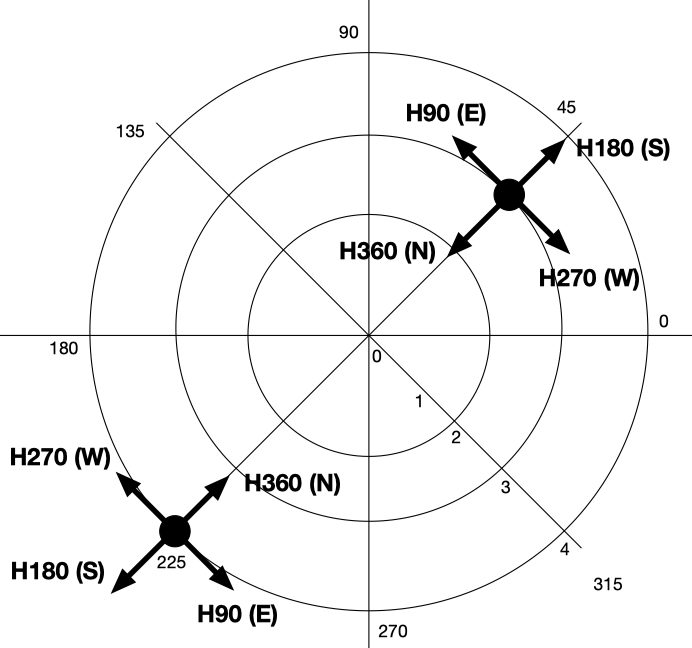
\includegraphics[width=0.5\textwidth]{report/figures/map.png}
\caption{\label{fig:map}A visualisation of a state space and its valid moves where $N=5$.}
\end{figure}

\subsubsection{Problem Definition}

\textbf{State space}: Corresponds to each position in the map. Each position is represented by a State object, as shown in the UML Class diagram in Appendix \ref{sec:uml_class_diagram}.\\

\textbf{Initial State}: Corresponds to the starting point defined by the user input. It is used to create the root node of the search tree. It is impossible to start on the pole (0,0).\\

\textbf{Goal}: To find the route from the initial state to the goal state while avoiding obstacles. For informed search algorithms, the goal includes finding the route with the minimal path cost. The goal state is stored in the Problem object, as shown in Appendix \ref{sec:uml_class_diagram}.\\

\textbf{Cost}: The cost to move across parallels ($N \rightarrow N+1$ or $N \rightarrow N-1$) is 1. The cost to move across meridians ($+45\degree$ or $-45\degree$) is $(2*\pi*d) / 8$.\\

\textbf{Successor Function}: The successor function generates the valid nodes that are adjacent to the current node, which are added to an ArrayList before being added to the frontier.

\subsubsection{System Architecture}

\paragraph{Class Design}

The system is designed with scalability and simplicity in mind. In order to avoid unnecessary code duplication, abstract classes are used to group common methods between the different search algorithms. An abstract class called \textit{GeneralSearch} organises all the general search methods such as \textit{successor}, \textit{goalTest}, \textit{isNodeInExploredSet} or \textit{findSolutionPathCost} into a single class. Abstract methods, such as \textit{makeNode}, which differ in implementation between informed and uninformed search algorithms, are then defined in this class and act as a template to implement in classes that extend \textit{GeneralSearch}.\\

Next, two abstract classes, \textit{InformedSearch} and \textit{UninformedSearch}, extend \textit{GeneralSearch}. In a similar fashion, they contain methods common to all concrete search algorithms, such as \textit{treeSearch}, \textit{expand} and \textit{removeFrontierNode}. They also override the \textit{makeNode} method declared in the \textit{GeneralSearch} abstract class, and declare their own abstract methods that will be extended by the concrete classes.\\

Finally, concrete classes extending the abstract classes are created. The \textit{BFS} and \textit{DFS} classes extend the \textit{UninformedSearch} abstract class, while the \textit{BestF} and \textit{AStar} classes extend the \textit{InformedSearch} abstract class. For a more detailed representation of the class inheritance used, see Appendix \ref{sec:uml_class_diagram}.\\

\paragraph{Data Structures}

Java offers a wide variety of data structures to use. The pros and the cons were weighed to choose which data structure to use for each aspect of the program. Concerning the frontier, two data structures are used. For uninformed search, a LinkedList is used, while for informed search, a PriorityQueue is used. LinkedLists are used because manipulation operation of adding/removing Nodes to/from the data structure is much cheaper than ArrayLists manipulation, which requires the entire array to be copied over to a new one to add or remove a single Node.\\

Additionally, custom objects are created to represent different aspects of the data and facilitate access. A Node object holds crucial information such as a pointer to a parent node (which are very useful when retracing the route found and calculating the route's cost), an action (H90, H180, H270, H360), a path cost, a depth and a State. States represent a location on the state space, including a parallel, an angle, an index to easily access it in the world, and a status to represent if it is the initial state (S), the goal state (G), the pole (0,0) (P) or an obstacle (X).

\paragraph{Map}

The world is represented as a LinkedList of Linkedlist of States.

\paragraph{Javadocs}

The entire system is covered by Javadoc comments. They can be compiled using the command below and opening the \textit{javadoc/index.html} file in a web browser:\\

\textit{javadoc -d javadoc A1src/*.java}

\begin{comment}
Key elements of implementation including any data structure or algorithm used if applicable. Remember to justify the mechanisms you have implemented as part of your solution.\\

Please do not include screenshots of your code, pseudo code can be used instead with relevant references to where this can be found in your code.\\

Motivate your choices: this can be done by considering why as well as how you have implemented the system in the way you did.
\end{comment}

\subsection{Evaluation}

todo

\begin{comment}
This section is about performance of the system. A critical analysis of the functionalities of your system and what can be improved. The role of this section is to show and demonstrate the qualities and limitations of your system such as how effectively or efficiently the system works under certain conditions.\\

Depending on the type of assignment, this section should include results of any evaluation performed at a large scale, for example a table/graph showing performance results.\\

Pros and Cons of your approach should also be discussed, and any component that could be improved.\\
\end{comment}

% -------------------------------------- 3 - TEST SUMMARY ------------------------------------------ 
\section{Test Summary}
\label{sec:test-summary}

This section is about correctness of the system. Include a table or a list of tests performed, with input and output where appropriate. The role of this part is to show that your system is working correctly. You could also include:

\begin{itemize}
    \item Screenshots of the outputs
    \item Small working examples
    \item Graphical representation of these working examples (etc)
\end{itemize}

% ---------------------------------------- 4 - CONCLUSION ------------------------------------------ 

\section{Conclusion}
\label{sec:conclusion}

List all the references you cite in your report and code.

% -------------------------------------------- APPENDIX -------------------------------------------- 

\newpage
\begin{appendices}

\section{UML Class Diagram}
\label{sec:uml_class_diagram}

The UML Class Diagram of the program, generated using yWorks \cite{yworks}.

\begin{sidewaysfigure}[ht]
\centering
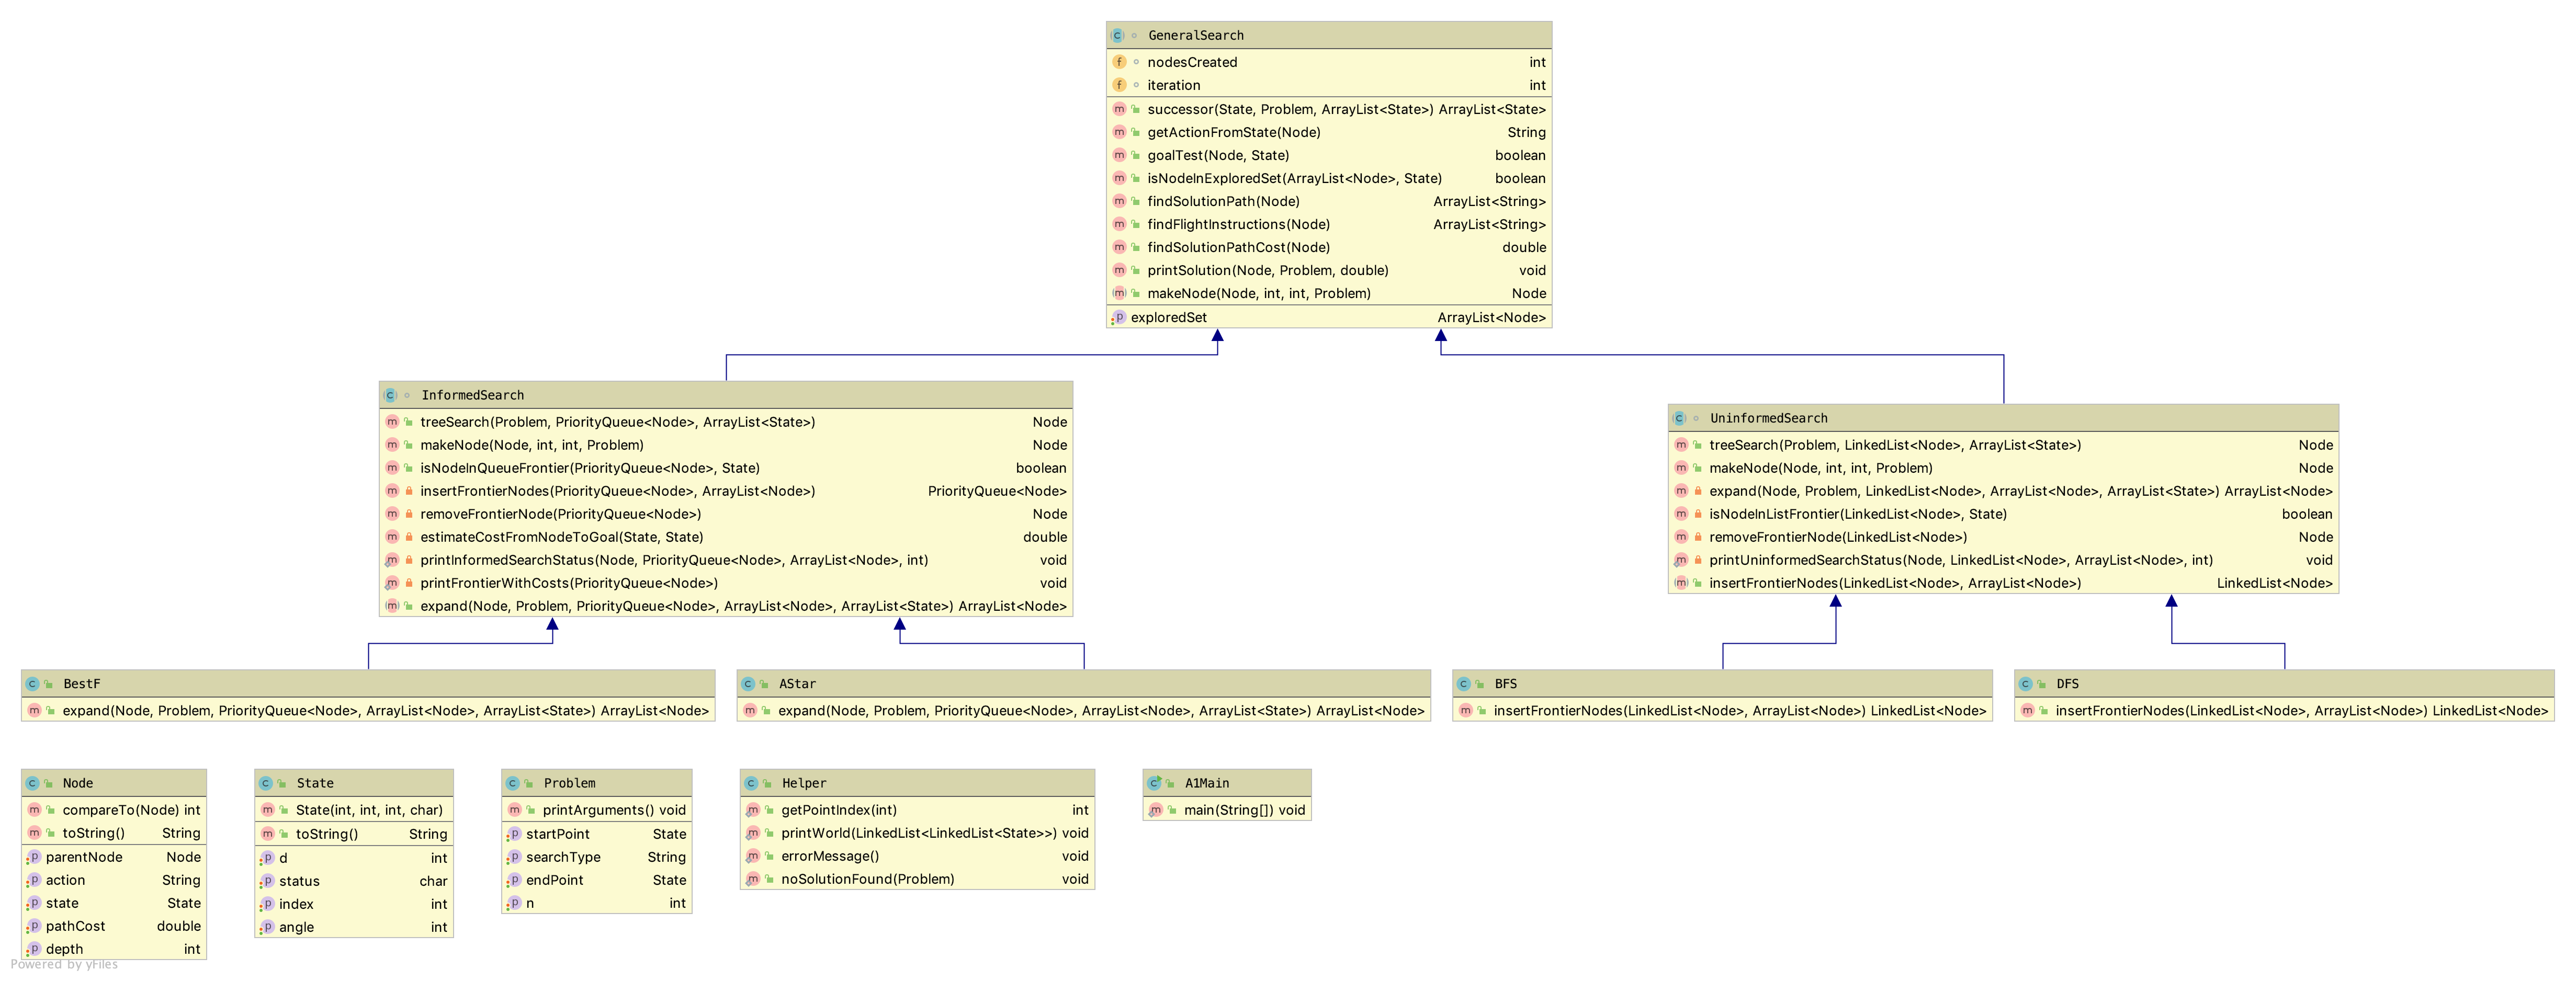
\includegraphics[width=\textwidth]{UML/UML_class_diagram.png}
{\label{fig:uml_class_diagram}}
\end{sidewaysfigure}

\newpage
\bibliographystyle{plain}
\bibliography{bibliography}

\end{appendices}
\end{document}